\documentclass[tikz]{standalone}

\usetikzlibrary{shapes}
\usetikzlibrary{angles}
\usetikzlibrary{calc} 

\usetikzlibrary{decorations.pathreplacing}
\usetikzlibrary{decorations.markings}
\usetikzlibrary{decorations.text}


% This bascially automates a \newcommand{<name>}{} to ensure
% that a command with the given <name> does not already exist
\providecommand*{\pgfmathsetnewmacro}[2]{%
    \newcommand*{#1}{}% Error if already defined
    \pgfmathsetmacro{#1}{#2}%
}%

\begin{document}

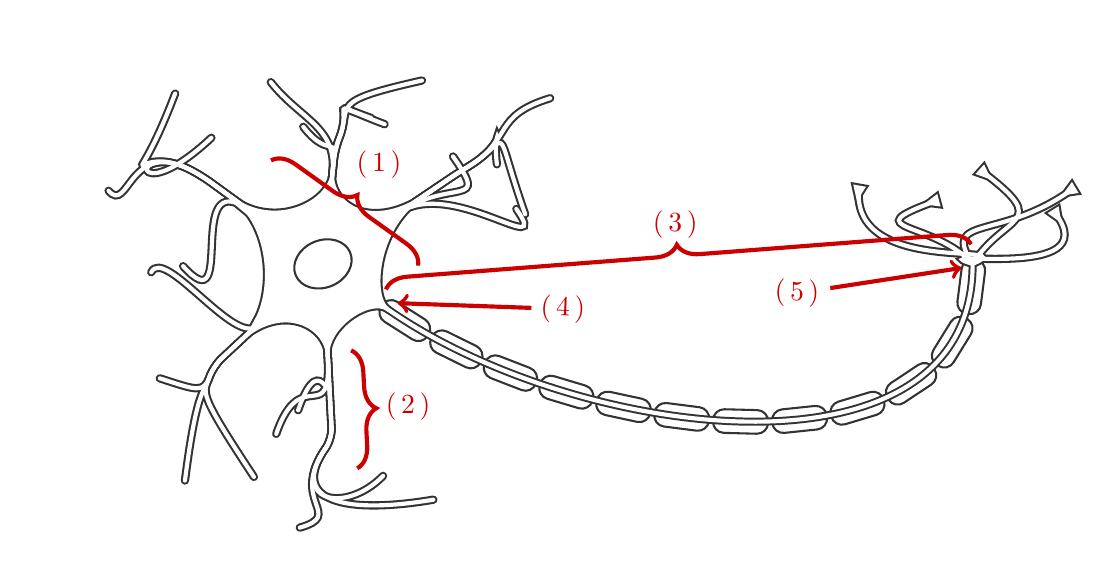
\begin{tikzpicture}[
        scale = 1.5,
        draw = black!80,
        fill = white,
        ]
    
\clip[use as bounding box] (-2.5,-2.5) rectangle (6.5,2);
%\draw[help lines] (-2.5,-3) grid (6,2);
%\draw[white,->] (0,-4) -- (0,4);
%\draw[white,->] (-3,0) -- (6,0);

% Random Num shit
\def\ranAngle#1{\pgfmathrandominteger{#1}{-75}{75}}
\def\ranLength#1{\pgfmathrandominteger{#1}{5}{15}}
\def\ranScale#1{\pgfmathrandominteger{#1}{-10}{10}}

% Colors
\newcommand*\neuronClr{black!80}


% Random number generation seed
%\pgfmathsetnewmacro\seed{220699}
%\pgfmathsetnewmacro\seed{04081999}
\newcommand*\seed{1669}
%\pgfmathsetnewmacro\seed{1984}
%\pgfmathsetnewmacro\seed{2356}
\pgfmathsetseed{\seed}

% Various constants
\pgfmathsetnewmacro\sh{5.0}                    %
\pgfmathsetnewmacro\w{8.0}                     %
\pgfmathsetnewmacro\bloatStr{0.5}              %
%\pgfmathsetnewmacro\armLen{1}                  %
%\ranLength{\armLen}             %
%\pgfmathsetnewmacro\pole{0.5}                  %
\ranLength{\pole}               %
\pgfmathsetnewmacro\axonLen{5.5}               %
\pgfmathsetnewmacro\tentLen{1/15}              %
\pgfmathsetnewmacro\neuronC{0.1}                     %
\pgfmathsetnewmacro\rx{0.25}                   %
\pgfmathsetnewmacro\ry{0.20}                   %
\pgfmathsetnewmacro\neuronAngle{45}                  %
\pgfmathsetnewmacro\linthicc{3pt}              %
\pgfmathsetnewmacro\linthic{1.5pt}     %
\pgfmathsetnewmacro\linthin{0.75pt}      %


% Angles for the polar coordinates, uses degrees for god knows what reason
%\pgfmathrandominteger{\rara}{0}{300}
\pgfmathsetnewmacro{\pI}{34}
\pgfmathsetnewmacro{\pII}{84}
\pgfmathsetnewmacro{\pIII}{144}
\pgfmathsetnewmacro{\pIV}{223}
\pgfmathsetnewmacro{\pVee}{273}
\pgfmathsetnewmacro{\pVI}{325}

% Shortcut for loop
\newcommand\forlist[1]{%
    \foreach \i in {\pI,\pII,\pIII,\pIV,\pVee,\pVI}{#1}%
    }

% Fixed points
\coordinate (O) at (0,0); % The origin
\coordinate (SC) at (\axonLen, 0.0); % The synaptic cleft potistion

% Some custom commands/shortcuts
% Cell "spikes"
\newcommand*\pcoord[2]{#1:#2}
\forlist{
    \pgfmathrandominteger{\armLen}{10}{15}
    \coordinate (P\i) at (\pcoord{\i}{\armLen/15});
    %\fill (P\i) circle (1.5pt);
    }
\coordinate (P\pVI) at (\pcoord{\pVI}{2/3});
\coordinate (AH) at (P\pVI);


\newcommand*\bloat[1]{#1:\bloatStr}
\newcommand*\contr[2]{(P#1) .. controls (\bloat{#1+\sh}) and (\bloat{#2-\sh}) .. }
    
\newcommand\aggcontr[5]{
            \contr{#1}{#2}
            \contr{#2}{#3}
            \contr{#3}{#4}
            \contr{#4}{#5}
            }
\newcommand*\axonPath{(P\pVI) to[out=\pVI, in=-90] (SC)}
\foreach \SIGN/\i in {-/1, +/2}{%
    \path \axonPath -- ([turn]\SIGN 45:0.75) coordinate (CL\i);
    }

% Axon mylene sheath decoration
\begin{scope}[decoration={markings,
                mark=between positions 0.03 and 1 step 0.75cm
                with { \node   [rectangle, 
                                rounded corners, 
                                fill = white, 
                                draw = \neuronClr,
                                inner sep=0pt,
                                minimum height=0.30cm,minimum width=0.7cm,
                                behind path,
                                transform shape] {};}}]
    \draw[postaction={decorate}, line width = 0.75pt]
        \axonPath;
\end{scope}

\newcommand\synCleft{
    \foreach \i in {-0.3,-0.15,0.4,0.8,1.4}{
        \pgfmathrandominteger{\slp}{-4}{12}
        \ranAngle{\srpI}
        \ranAngle{\srpII}

        \def\tmp{90+\srpI}
        \draw[line cap = butt] ($(CL1)!\i!(CL2)$)+(95:\slp/20) node[fill, draw, scale = 0.20, isosceles triangle, rotate = {-\tmp}] {} .. controls +(180+95+\srpI:0.75) and +(95+\srpII:0.5)  .. (SC);
        }
    }

    % Cell body
    % gives the juicy looking cell body
    % Generates random angles for the branching arms
    \newcommand\limbConstruct{
        \ranAngle{\ra}
        \ranAngle{\rb}
        \ranAngle{\rc}
        \ranAngle{\rangA}
        \ranAngle{\rangB}
        \ranAngle{\rangC}
        \ranLength{\rla}
        \ranLength{\rlb}
        \ranLength{\rlc}
        \ranLength{\rext}
        \ranLength{\rarm}
        
        \foreach \v in {\ra:\tentLen*\rla,
                        \rb:\tentLen*\rlb,
                        \rc:\tentLen*\rlc
                        }{
            \draw [line cap = round, rounded corners]
                (P\i) -- ([turn]0:\rext/20) 
                .. controls 
                ([turn]\rangB :\rarm/20) and 
                ([turn]\rangC:\rarm/20) .. 
                %to[out=\rangB, in=\rangC]
                ([turn]\v) 
                %node[ draw, isosceles triangle, rotate = \rangC, scale = 1]{}
                ;
            }
        \foreach \v in {\i+\rb:\tentLen*\rlc,
                        \i+\rc:\tentLen*\rla
                        }{
            \draw [line cap = round, rounded corners]
                (PP\i) 
                .. controls 
                ([turn]0:\rarm/20) and 
                +(\rangA:\rarm/20)  .. ([turn]\v) 
                %node[fill,draw, isosceles triangle, rotate = 180+\rangA, scale = 0.00005]{}
                ;
            }}

    % Builds and outlines the Neuron
\foreach \COLOR/\THICKNESS in {black!80/\linthicc, white/\linthic}{
    \begin{scope}[\COLOR, line width = \THICKNESS pt] 
        \pgfmathsetseed{\seed}
        \foreach \i in {\pI,\pII,\pIII,\pIV,\pVee}{
            \draw%
                (P\i) -- (\i:\pole/13) coordinate (PP\i);
            \limbConstruct
            }
        \filldraw%
            \aggcontr{\pI}{\pII}{\pIII}{\pIV}{\pVee} 
            (P\pVee) .. controls (\bloat{\pVee+\sh}) and (\bloat{\pVI}) ..              
            (P\pVI) .. controls (\bloat{\pVI}) and (\bloat{\pI-\sh}) ..
            cycle;
        \ifx\neuronClr\COLOR%  
            \draw%
            [line width = 1.95*\linthic]\axonPath;%
            \fill (P\pVI) circle;%
            \else 
                {\draw% 
                [line width = \linthic]\axonPath;%
                \fill (P\pVI) circle;}
            \fi
        \synCleft
    \end{scope}
    }

\draw[rounded corners, rotate = 23, line width = \linthin]  
        (0,0) ellipse [x radius=\rx cm, y radius=\ry cm];
%\draw[white,rounded corners, rotate = 90]  
%        (45:\rx) rectangle (225:\rx);

% Labeling
\begin{scope}[opacity = 1, red!80!black, line width = 1.5pt]
    
    % Soma label
    \pgfmathsetnewmacro{\somaSlope}{(\pIII + \pVI)/2}
    \path (P\pIII) -- +(\somaSlope:-0.45) coordinate (Sa);
    \path (P\pVI)  -- +(\somaSlope:-0.45) coordinate (Sb);

    \pgfmathsetnewmacro{\somaTextSlope}{\somaSlope + 90}
    \draw[decoration ={brace, amplitude = 8}, decorate] 
        (Sa) -- (Sb) node[midway, sloped, allow upside down= true, 
        above, yshift = 0.3cm] { \rotatebox{-\somaTextSlope}{$\left(\, 1 \,\right)$}};

    % Dendrite label
    \path (P\pVee) -- ++(0:0.20) coordinate (Da);

    \draw[decoration ={brace, amplitude = 8}, decorate] 
            (Da) -- ($(Da)!1!(Da)+(\pVee:1)$) 
            node[midway, sloped, 
            above, yshift = 0.25cm, allow upside down= true] { \rotatebox{-\pVee}{$\left(\, 2 \,\right)$} };

    % Axon label
    \pgfmathsetnewmacro{\axonTextSlope}{ atan2( (11/15) * sin(\pVI), \axonLen * cos(0)) }
    \draw[decoration ={brace,amplitude = 8, raise = 0.25cm}, decorate] 
            (P\pVI) -- (SC) node[midway, sloped, 
            above, yshift = 0.45cm] {\rotatebox{\axonTextSlope}{$\left(\, 3 \,\right)$}};    
    
    % Axon Hill label
    \draw[<-] 
            (AH)+(30:1mm) node (AHpoint) [circle] {} -- +(0:1.5) node[align=left, pos = 0.99, sloped, 
            fill = white] {\rotatebox{0}{$\left(\, 4 \,\right)$}};   

    % Synaptic Cleft label
    \pgfmathsetnewmacro{\axonTerminalTextSlope}{pi/2 *((4 - \axonLen)/(-0.25 - 0.0))}
    \draw[<-] 
            (SC)+(200:1mm) node (SCpoint) [circle] {} -- (4,-0.25) node[align=left, pos = 0.99, sloped, 
            fill = white] {\rotatebox{-\axonTerminalTextSlope}{$\left(\, 5 \,\right)$}};   
\end{scope}

%\draw (-10,0) to (10,0);
%\draw[yshift = 0.25cm] (-10,0) to (10,0);
\end{tikzpicture}     

\end{document}